\documentclass[a4paper, 12pt]{article}

% Работа с русским языком ======================================================

\usepackage[T2A]{fontenc}             % Кодировка
\usepackage[english, russian]{babel}  % Локализация и переносы
\usepackage[utf8]{inputenc}           % Кодировка исходного текста
\usepackage{indentfirst}              % Красная строка в первом абзаце

% Оформление страницы ==========================================================

% Поля

\usepackage{geometry}
\geometry{top=25mm}
\geometry{bottom=30mm}
\geometry{left=20mm}
\geometry{right=20mm}

\linespread{1.5} % Коэффициент межстрочного интервала

% Колонтитулы

\usepackage{titleps}
\newpagestyle{main}{
	\setheadrule{0.4pt}
	\sethead{left}{center}{right}
	\setfootrule{0.4pt}
	\setfoot{left}{\thepage}{right}
}

\pagestyle{main}

% Работа с картинками ==========================================================
\usepackage{graphicx} % Для вставки рисунков

% Математика ===================================================================

\usepackage{amsmath}
\usepackage{amsfonts}
\usepackage{mathtools}

\newcommand{\deriv}[2]{\frac{\partial #1}{\partial #2}}
\newcommand{\R}{\mathbb R}

\renewcommand{\phi}{\varphi}

\DeclareMathOperator{\Kerr}{Ker}
\DeclareMathOperator{\Ree}{Re}
\DeclareMathOperator{\Imm}{Im}

% Здесь звёздочка перевод нижний индекс под оператор в формуле только на лной строке
\DeclareMathOperator*{\argmax}{argmax}

% Бинарная операция
\newcommand{\percent}{\mathbin{\%}}

\usepackage{amsthm}    % Создание теорем
\theoremstyle{plain}   % {plain, definition, remark}
\newtheorem{theorem}{Теорема}[section]
\newtheorem{corollary}{Следствие}[theorem]

% Звёздочка отменяет нумерацию
\newtheorem*{definition}{Определение}

% ==============================================================================

\newenvironment{myenv}
    {\begin{center}\bfseries}
    {\end{center}}

\usepackage{hyperref}

\usepackage{tikz}
\usetikzlibrary{calc,intersections,through,backgrounds}
\usetikzlibrary{graphs}
\usetikzlibrary{shapes.geometric}
\usepackage{tkz-euclide}

% Листинги

\usepackage{listings}
\usepackage{xcolor}

\definecolor{mygreen}{rgb}{0.0, 0.15, 0.05}

\lstdefinestyle{mystyle}
{
% backgroundcolor=\color{black!5}, % set backgroundcolor
  basicstyle=\footnotesize,% basic font setting
  breaklines=true,
  commentstyle=\color{mygreen},
  frame=single,
  keywordstyle=\color{blue}\textbf,
  language=C++,
  numbers=left,
  extendedchars=\true
}

\lstset {style=mystyle}

% Для вставки текстового файла с переносом строк
\usepackage{verbatim}

% Для задания межстрочного интервала
\usepackage{setspace}

\begin{document}
	Привет, мир!\\
	Курс: \href{https://www.youtube.com/watch?v=JFEM_HxhNnY&list=PL4_hYwCyhAvZtx63FR9d5_K0GMWF1XUc6}{ссылка}

	Читателю предлагается проверить, что выполнено равенство $2 + 2 = 4$
	\[ 3 + 6 = 9\]

	\textbf{Жирный текс}
	\textit{Курсивный текс}
	\textbf{\textit{Жирный и курсивный текст}}

	{ \bfseries \itshape \Large Какой-то текст.} А тут обычный текст.

	\Huge A
	\LARGE A
	\Large A
	\large A
	\normalsize A
	\small A
	\dots

	Cкобки
	\[ (\frac{\pi}{2}),
	   \big( \frac{\pi}{2} \big),
	   \bigg( \frac{\pi}{2} \bigg),
	   \left( \frac{\pi}{2} \right),
	   \left\lfloor \frac{\pi}{2} \right\rfloor,
	   \left\lceil \frac{\pi}{2} \right\rceil,
	   \bigg\lceil  \frac{\pi}{2} \bigg\rceil
	\]

	Новая строка.
	\[  \int_{- \infty}^{+ \infty} e^{- \frac{x^2}{2}} dx = \sqrt{2 \pi} \]

	Пример таблицы \\
	\begin{tabular}{||c|c|||r|l||}
		1 & 2 & aligned & aligned \\
		\hline
		3 & 4 & to the right & to the left \\
	\end{tabular}

    \vspace{10pt}

    Таблица с визардом \\
    \begin{tabular}{|c|c|c|}
	    \hline
	    C1 & C2 & C2 \\
	    \hline
	    Value-1 & \multicolumn{2}{c|}{Value-2Value-3} \\
	    \hline
    \end{tabular}

    \vspace{10pt}

    А вот рисунок \\

    \begin{center}
  	    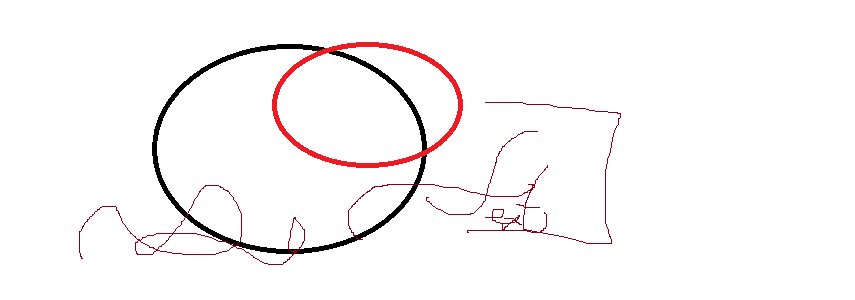
\includegraphics[width=0.8\textwidth]{img/picture}
    \end{center}

    $\deriv{f}{x}$
    $\R$

    Кастомный оператор: $\Kerr x = A$

    $\Re (z) + \Im(z)$ \hspace{10pt}   $\Ree(z) + \Imm(z)$

    \[ \argmax_{x \in [0;1]} f = 0 \]

    Но внутри строки $\argmax_{x \in [0;1]} f = 0$

    Бинарная операция: $A \percent B$

    itemize:
    \begin{itemize}
        \item Пункт 1
        \item Пункт 2
    \end{itemize}

    enumerate:
    \begin{enumerate}
    	\item Первый пункт
    	\item Второй пункт
    \end{enumerate}

    Докажем, что $ a = b \leftrightarrow b = a $ для любых $a,b \in \mathbb{R}$
    \begin{itemize}
    	\item[$\leftarrow$] Очевидно
    	\item[$\rightarrow$] Тривиально
    \end{itemize}

    Создание теорем

    \section{Первый раздел}

    \begin{theorem}Текст.\end{theorem}
    \begin{theorem}Еще текст.\end{theorem}
    \begin{proof}Тривиально.\end{proof}
    \begin{corollary}Еще текст\end{corollary}
    \begin{definition}Что-то новое\end{definition}

    \begin{myenv}
    	Моё окружение
    \end{myenv}

    Шрифты в математическом окружении\\
    \begin{tabular}{|c|c|c|}
	    \hline
	    Команда & Пример & Результат \\
	    \hline
	    \textbackslash mathbb & x \textbackslash in \textbackslash mathbb R & $ x \in \mathbb R $ \\
	    \hline
	    \textbackslash mathbf & \textbackslash mathbf \{Ax\} = \textbackslash b & $\mathbf{Ax} = \mathbf b$ \\
	    \hline
	    \textbackslash mathrm & \textbackslash phi \textbackslash in \textbackslash mathrm \{GL\}(V) & $ \phi \in \mathrm{GL}(V) $ \\
	    \hline
	    \textbackslash mathsf & \textbackslash mathsf E \textbackslash xi < + \textbackslash infty & $ \mathsf E \xi < + \infty $ \\
	    \hline
	    \textbackslash mathcal & \textbackslash psi \textbackslash in \textbackslash mathcal L(V)  & $ \psi \in \mathcal L(V) $ \\
	    \hline
    \end{tabular}

    \vspace{10pt}

    Пределы

    Внутри строки $ e^x = \sum_{n=0}^{+ \infty} \frac{x^n}{n!} = \sum\limits_{n=0}^{+ \infty} \dfrac{x^n}{n!} $

    На новой строке:
    \[ e^x = \sum_{n=0}^{+ \infty} \frac{x^n}{n!} = \sum\limits_{n=0}^{+ \infty} \dfrac{x^n}{n!} \]

    $ S = a_1 \cdot a_2 \cdot a_3 \dots a_n  $

    \[ \phi \xleftrightarrow{eeeeeee} A  \]
    \[ \phi \xleftrightarrow[rrrrrrr \text{просто текст}]{eeeeeee} A  \]

    Знаки над символами

    \begin{tabular}{|c|c|c|c|}
    	\hline
    	Короткий вариант & Результат & Длинный вариант & Результат \\
    	\hline
    	\$ \textbackslash dot a \$ & $ \dot a $ & \texttwelveudash & \texttwelveudash \\
    	\hline
    	\$ \textbackslash ddot a \$ & $ \ddot a $ & \texttwelveudash & \texttwelveudash \\
    	\hline
    	\$ \textbackslash mathring a\$ & $ \mathring a $ & \texttwelveudash & \texttwelveudash \\
    	\hline
    	\$ \textbackslash hat a \$ & $ \hat a $ & \$ \textbackslash widehat\{AB\} \$ & $ \widehat{AB} $ \\
    	\hline
    	\$ \textbackslash tilde a \$ & $ \tilde a $ & \$ \textbackslash widetilde \{AB\} \$ & $ \widetilde{AB} $ \\
    	\hline
    	\$ \textbackslash bar a \$ & $ \bar a $ & \$ \textbackslash overline \{AB\} \$ & $ \overline{AB} $ \\
    	\hline
    	\$ \textbackslash vec a \$ & $ \vec a $ & \$ \textbackslash overrightarrow \{AB\} \$ & $ \overrightarrow{AB} $ \\
    	\hline

    \end{tabular}

    Equation environment

    \begin{equation}
    	ax = b
    \end{equation}

    Align environment

    \begin{align*}
    	a_1x_1 &= b_1 \\
    	a_2x_2 &= b_2 \\
    	&\dots        \\
    	a_nx_n &= aaaaaaaaaaaa
    \end{align*}

    \newpage

    Gather environment

    \begin{gather*}
    	a_1x_1 = b_1 \\
    	a_2x_2 = b_2 \\
    	\dots        \\
    	a_nx_n = aaaaaaaaaaaa
    \end{gather*}

    \begin{align*}
    \label{eq:3n}
    	F = \frac{dp}{dt} \tag{III ЗН}
    \end{align*}

    Система линейных уравнений
    \begin{align*}
    \begin{cases}
    	a_1x + b_1y = c_1, \\
    	a_2x + b_2y = c_2
    \end{cases}
    \end{align*}

    Матрица
    \begin{align*}
    \begin{pmatrix}
    	a & b \\
    	c & d
    \end{pmatrix}
    \end{align*}

    Квадратная матрица $ n \times n $:
    \begin{align*}
    \begin{pmatrix}
    	a_{11} & a_{12} & \cdots & a_{1n} \\
    	a_{21} & a_{22} & \cdots & a_{2n} \\
    	\vdots & \vdots & \ddots & \vdots \\
    	a_{n1} & a_{n2} & \cdots & a_{nn}
    \end{pmatrix}
    \end{align*}

    \newpage

    Следующий раздел - ссылки
    \eqref{eq:3n} \pageref{eq:3n} \ref{eq:3n}

    Ссылки на формулы рекомендовано начинать с eq:, на рисунки - fig:

    \href{https://www.google.com/}{google.com}

    сноска \footnote{сноска с английского}
    Ещё одна сноска \footnote{сноска номер 2 \label{footnote}}

    А вот ссылка на сноску №\ref{footnote}

    Рисование с tikz

    \tikz \draw (0pt, 0pt) -- (1in, 8pt);

    next?

    \tikz \fill [orange] (1ex, 1ex) circle (1ex);

    Путь - основной блок всех рисунков в TikZ. Он состои из точек (x, y) и -- Весь код помещается в окружение tikxpicture

    \begin{tikzpicture}
      \draw (0, 0) -- (0, 1) -- (1, 2);
    \end{tikzpicture}

    Кружочки

    \tikz \draw circle(10pt);
    \tikz \draw ellipse(20pt and 10pt);
    \tikz \draw [rotate=30] ellipse(20pt and 10pt);

    Сетка

    \tikz \draw [xstep=0.4, ystep=0.5] (0, 0) grid(2,2);

    Комбинации

    \begin{tikzpicture}
    	\draw (0, 0) circle(10pt);
    	\draw (0, 0) ellipse(20pt and 10pt);
    	\draw [rotate=30] (0, 0) ellipse(20pt and 10pt);
    	\draw [step=.5cm, gray, very thin] (-1.4, -1.4) grid(1.4, 1.4);
    \end{tikzpicture}

	Свой стиль:

	\tikzset{help lines/.style={very thin, gray}}
	\tikz \draw [step=.5cm, help lines] (-1.4, -1.4) grid(1.4, 1.4);

	\begin{tikzpicture}
		\draw [fill=gray!10, thin, densely dashed ] (0, 0) -- (1, 0) -- (1, 1) -- (0, 1) -- cycle ;
		\draw [fill=blue!10, thick, loosely dotted] (2, 0) -- +(10:2) arc (0:30:2) --cycle;
	\end{tikzpicture}

	Стрелочки

	\tikz \draw [->] (0, 0) -- (2, 0);
	\begin{tikzpicture} [scale=2, >=stealth]
		\draw [->] (0, 0) arc (180:30:10pt and 20pt);
		\draw [-latex] (3, 0) -- +(1, 0);
		\draw [<<-, very thick] (1, 0) -- (1.5cm, 10pt) -- (2cm, 0pt) -- (2.5cm, 10pt);
	\end{tikzpicture}

	Про точки

	\tikz \coordinate (A) at (0, 0);
	\tikz \draw (A) circle(1);

	\begin{tikzpicture}
		\coordinate (A) at (0, 0);
		\coordinate (B) at (0.1, 0.3);
		\node[draw, circle through=(A)] at (B) {};
	\end{tikzpicture}

	Упрощаем вычисления I

	\begin{tikzpicture}
		\coordinate (A) at (0, 0);
		\coordinate (B) at (60:1.5);
		\coordinate (C) at (30:3);
		\coordinate (D) at ($(A) + (2, -1)$);

		\draw [dashed] (A) -- (A |- B) -- (B);
		\draw [dotted] (B) -- (D) -- (C);
		\draw (B) -- ($(D)!(B)!(C)$);
		\draw (A) -- ($(B)!0.5!(D)$);

		\tkzLabelPoint[](A){A}
		\tkzLabelPoint[](B){B}
		\tkzLabelPoint[](C){C}
		\tkzLabelPoint[](D){D}
		\tkzMarkAngle [mark=,arc=ll,size=0.3](C,D,B);
		\tkzLabelAngle[pos=0.6](C,D,B) {$\alpha$};
		\tkzMarkRightAngle(D,A,B);
		\tkzMarkSegment[mark=|](A,A |- B);
	\end{tikzpicture}

	Упрощаем вычисления II

	\begin{tikzpicture}
		\coordinate (A) at (2, 2);
		\tkzLabelPoint[](A){A}

		\coordinate (B)  at (4, 4);
		\tkzLabelPoint[](B){B}

		\draw [name path=A--B] (A) -- (B);

		\node (D) [name path=D, draw, circle through=(B), label=left:$D$] at (A) {};

		\node (E) [name path=E, draw, circle through=(A), label=right:$E$]  at (B) {};

		\path [name intersections={of=D and E,
		       by={[label=above:$C$]C,
	                [label=below:$C'$]C'}}];

        \draw [name path=C--C', color=red] (C)--(C');

        \path [name intersections={of=A--B and C--C', by=F}];
        \tkzLabelPoint[](F){F}
	\end{tikzpicture}

\end{document}}
